\chapter{Results}\label{ch:results}

In this chapter, we discuss the application of the IM-SRG
to calculate the ground-state energies of two different fermionic systems.
The first is the pairing Hamiltonian,
which has been used to study pairing effects in finite and infinite systems.
We use this well-studied system as a benchmark for our numerical implementation,
as its small modelspace allows for calculations to complete relatively quickly.
The second is ${}^4\text{He}$,
the lightest closed-shell nucleus,
in a restricted modelspace in the IM-SRG(2).
The results of our implementation are then compared
against those from another open-source IM-SRG(2) library.

\section{The pairing Hamiltonian}

The pairing Hamiltonian is given by
\begin{equation}\label{eq:pairing_hamiltonian}
  H = \delta \sum_{p\sigma} (p - 1) \crea{p\sigma} \annih{p\sigma}
  - \frac{g}{2} \sum_{p q} \crea{p+}\crea{p-} \annih{q-} \annih{q+}\,,
\end{equation}
where we have equally-spaced two-fold degenerate levels indexed by the quantum number $p$
and an attractive (for $g > 0$) pairing interaction.
Cooper first considered this Hamiltonian in 1956~\cite{Coop56pairing_hamiltonian},
which led to the successful Bardeen-Cooper-Schreifer (BCS) theory of superconductivity~\cite{Bard57bcs}.
The exact eigenvalues of the pairing Hamiltonian were given by Richardson in 1963,
where the solutions are obtained via the solution of the non-linear coupled Richardson equations~\cite{Rich63pairing_hamiltonian}.

We focus on a restricted case where $p=1,\ldots,4$ and $\delta=1\mev$,
and we vary the strength of the pairing interaction $g$.
We are interested in the ground state of four fermions,
for which our reference state is the state with the two lowest levels completely filled,
\begin{equation}\label{eq:pairing_hamiltonian_reference}
  \refgnd = \crea{2-}\crea{2+}\crea{1-}\crea{1+}\ket{0}\,.
\end{equation}
This system has a couple of useful properties:
First, the number of single-particle states is only eight,
making the IM-SRG(3) calculation relatively tractable.
Additionally, one can increase the number of levels $p_{\text{max}}$ easily
to get a handle on the performance for larger single-particle basis sizes.
Second, in addition to the available exact solution,
this system is easy to construct and diagonalize in the basis
of the reference state and its particle-hole excitations,
\begin{equation}
  \{\refgnd, \refhp{ij}{ab}, \refhp{ijkl}{abcd} \}\,,
\end{equation}
where the odd number particle-hole excitations do not contribute
as Eq.~\ref{eq:pairing_hamiltonian} only couples pairs.
This makes it easy to obtain an exact solution with which to compare the IM-SRG(2)
and IM-SRG(3) solutions.
Finally, after normal ordering the Hamiltonian with respect to our reference state,
we find that $\hnoone$ is diagonal,
meaning our reference state is the canonical Hartree-Fock reference state
with the Hartree-Fock energy $\hnozero=E_{\text{HF}}=2 - g$.
This means the IM-SRG evolution must only bring in correlation corrections to the energy
without needing to overcome any reference state deficiencies.

\begin{figure}[t]
  \centering
  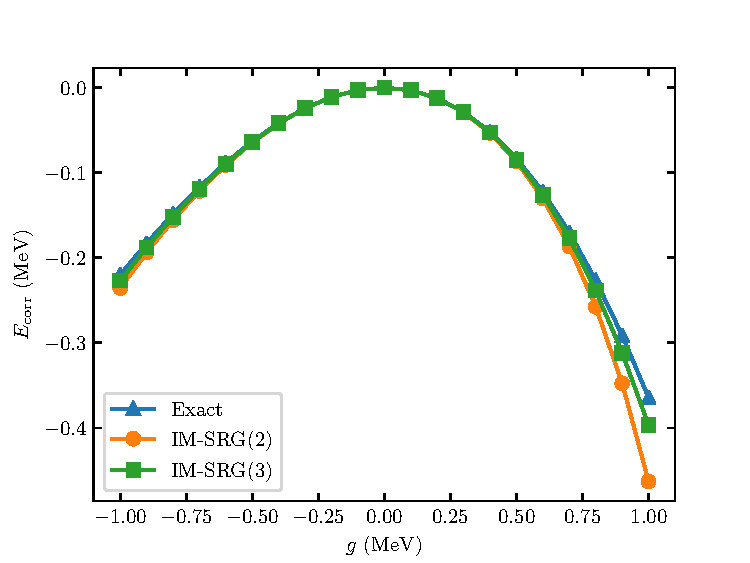
\includegraphics[width=0.9\textwidth]{proposal/doc/images/pairing_ham_imsrg3.pdf}
  \caption[
    The correlation energy $E_{\text{corr}}$ for the solution of the pairing Hamiltonian
    obtained via exact diagonalization,
    IM-SRG(2), and IM-SRG(3)
    for $-1 \le g \le 1$.
  ]{
    The correlation energy $E_{\text{corr}}$ for the solution of the pairing Hamiltonian
    obtained via exact diagonalization,
    IM-SRG(2), and IM-SRG(3)
    for $-1 \le g \le 1$.
    Exact diagonalization results obtained using code published with Ref.~\cite{Liet16lecnotesphysics}.
  }\label{fig:pairing_hamiltonian_fig}
\end{figure}

Thus, we are interested in the correlation energy obtained by the IM-SRG(2) and IM-SRG(3) solutions,
defined as
\begin{equation}
  E_{\text{corr}} = E(\infty) - E(0)\,.
\end{equation}
This is plotted in Fig.~\ref{fig:pairing_hamiltonian_fig} for $-1 \le g \le 1$.
We find generally good agreement between the IM-SRG correlation energy
and the exact correlation energy,
with the exception of the region for $0.5 \le g \le 1$.
Here, the IM-SRG(3) calculation improves upon the relatively large error in the IM-SRG(2)
correlation energy,
which in Ref.~\cite{Herg16imsrglecnotes}
was explained as being due to an overcounting in the fourth-order diagrams in MBPT
by a factor of 1/2 present in the IM-SRG(2) truncation.
It seems that this overcounting at fourth-order is lifted in the IM-SRG(3)
replaced by some overcounting at a higher MBPT order,
where the contributions are smaller in magnitude.
We note here that our results for IM-SRG(2) match exactly with those from Ref.~\cite{Herg16imsrglecnotes}.

\section{\texorpdfstring{${}^4\text{He}$}{Helium-4}}

The second system we consider here is ${}^4\text{He}$,
the lightest closed-shell nucleus.
Before we begin a discussion about the details of the system,
a few comments are in order.
The following calculation is restricted to a very small modelspace,
one insufficient to achieve converged results for observables.
This is because our implementation does not take advantage of the rotational invariance
of spherically symmetric systems,
that is, that the normal-ordered two- and three-body Hamiltonians
are diagonal in $J$ and $\mathcal{J}$
and independent of $M_{J}$ and $M_{\mathcal{J}}$.
The exploitation of the symmetries leads to so-called $J$-scheme IM-SRG flow equations.
The current results are a benchmark implementation for the IM-SRG(2)
that are compared against an existing IM-SRG(2) $J$-scheme implementation~\cite{Stro15imsrgcpp}.
This serves as an additional validation of our implementation
in addition to the results for the pairing Hamiltonian.
The current implementation will serve as a benchmark
against which we can compare our $J$-scheme IM-SRG(3) implementation,
which will be the focus of the next phase of this project.

As input into our calculation, we start with the intrinsic $A$-body Hamiltonian
with only an initial two-body interaction,
\begin{equation}
  H_{\text{int}} = T_{\text{int}} + \twobodyop{V}\,,
\end{equation}
with the intrinsic kinetic energy
\begin{align}
  T_{\text{int}} &= T - T_{\text{cm}} \\
                 &= \left(1 - \frac{1}{A}\right) \sum_{i} \frac{p_{i}^{2}}{2m}
                 - \frac{1}{A}\sum_{i<j}\frac{p_{i} \cdot p_{j}}{m}\,.
\end{align}
We note that the first term gives us our one-body Hamiltonian
and the second term contributes to the two-body Hamiltonian along with $\twobodyop{V}$~\cite{Herg09intrinsicham}.

We work in the single-particle harmonic-oscillator basis
at several different values of $\hbar \Omega$
(see Section~\ref{sec:sp_ho}),
with the single-particle states
\begin{equation}
  \ket{n_a (l_a s_a) j_a m_{j_a} t_a m_{t_a}} \equiv \ket{\alpha_a}\,,
\end{equation}
where $s_a=1/2$ and $t_a=1/2$.
A natural ordering of these states is according to their energy quantum number,
$e = 2  n + l$.
For the following calculation, we truncate the single-particle basis at $\emax=2$.
The resulting size of our single-particle basis is $N=40$.
As our reference state for ${}^4\text{He}$ we choose to fill the four $e=0$ HO states,
the most reasonable choice to target the ground state
without solving for and transforming to the Hartree-Fock basis.

\begin{figure}[t]
  \centering
  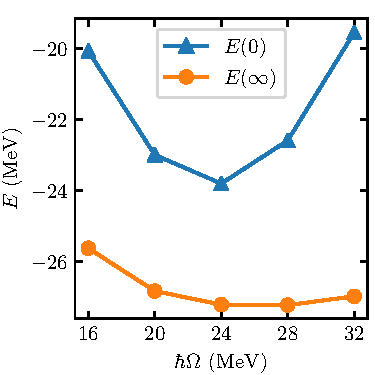
\includegraphics[width=0.45\textwidth]{proposal/doc/images/he4_imsrg2_energies.pdf}
  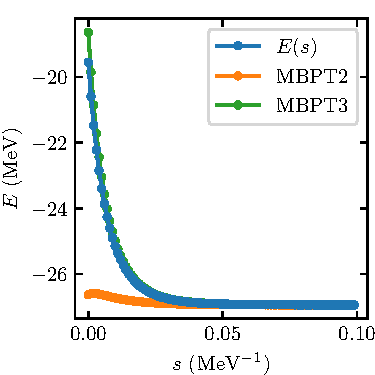
\includegraphics[width=0.45\textwidth]{proposal/doc/images/he4_imsrg2_flow.pdf}
  \caption[
    The left panel shows $E(0)$ and $E(\infty)$
    for an IM-SRG(2) calculation of ${}^4\text{He}$
    for $\hbar \Omega$ ranging from $16\mev$ to $32\mev$.
    The interaction used is the EM NN interaction
    with a regulator cutoff $\Lambda=500\mev$
    and SRG-evolved to $\lambda=1.8\invfm$.
    The right panel shows the flowing energy $E(s)$
    along with the energy with second- and third-order MBPT corrections included
    for $\hbar \Omega=32\mev$.
  ]{
    The left panel shows $E(0)$ and $E(\infty)$
    for an IM-SRG(2) calculation of ${}^4\text{He}$
    for $\hbar \Omega$ ranging from $16\mev$ to $32\mev$.
    The interaction used is the EM NN interaction
    with a regulator cutoff $\Lambda=500\mev$
    and SRG-evolved to $\lambda=1.8\invfm$~\cite{Ente03n3lonn}.
    The right panel shows the flowing energy $E(s)$
    along with the energy with second- and third-order MBPT corrections included
    for $\hbar \Omega=32\mev$.
  }\label{fig:imsrg2_he4_results}
\end{figure}

For $\twobodyop{V}$, we use the EM NN potential from Ref.~\cite{Ente03n3lonn} at N3LO
with a regulator cutoff at $\Lambda=500\mev$ and SRG-evolved to $\lambda=1.8\invfm$.
This potential has been shown to reproduce experimental binding energies
across the nuclear chart very well~\cite{Hebe20habi}.
The results from normal ordering our Hamiltonians at the different $\hbar \Omega$
with respect to our HO reference state
and evaluating the IM-SRG(2) evolution are shown
in the left panel of Fig.~\ref{fig:imsrg2_he4_results}.
We find that the unevolved energy $E(0)$,
that is, the energy expectation value of the reference state,
is already good to within 30\% of the exact result,
a consequence of the SRG-softened interaction we are using.
Still, the IM-SRG evolution absorbs up to $8\mev$ of correlation energy into the ground-state energy.
We also find that our implementation agrees with the implementation from Ref.~\cite{Stro15imsrgcpp}
to within $10^{-5}\mev$.

In the right panel of Fig.~\ref{fig:imsrg2_he4_results},
we show the flowing ground-state energy
as well as the ground-state energy with second- and third-order MBPT corrections.
We find that these corrections vanish as the correlations are absorbed into the ground-state energy,
indicating that we are achieving the desired decoupling.
We emphasize once again that these results are intended to be interpreted as validation
(for example, as a nuclear-like toy model)
and not as physically meaningful.
We consider the agreement between our implementation and that of Ref.~\cite{Stro15imsrgcpp}
to be \textit{a posteriori} evidence of the correctness of our implementation.

